\graphicspath{ {./Figure/Figure12/}}
\begin{figure}
  \centering

  \hspace*{\fill}
  \subfigure[]{\label{subfig:10a}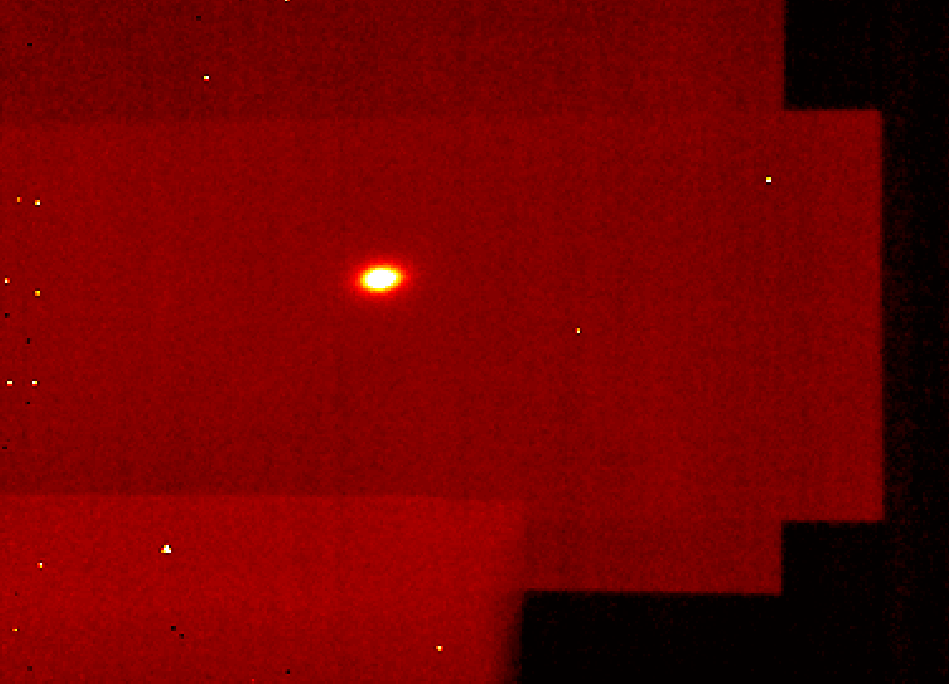
\includegraphics[width=0.3\linewidth]{fig10aa.png}} \hfill
  \subfigure[]{\label{subfig:10b}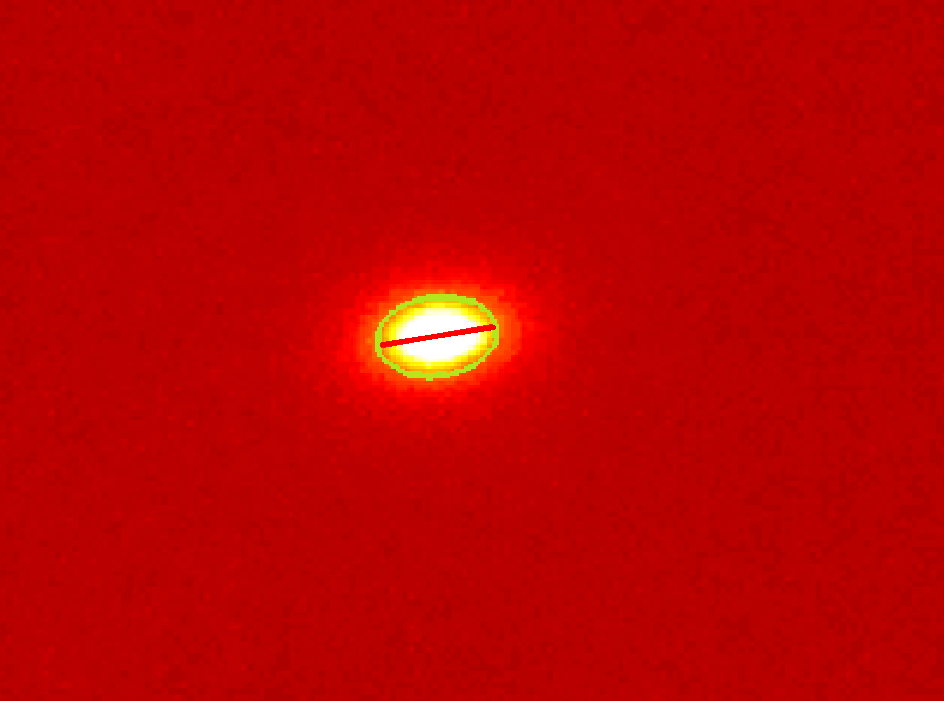
\includegraphics[width=0.3\linewidth]{fig10bb.png}} 
  \hspace*{\fill} \\ \hspace*{\fill}
  \subfigure[]{\label{subfig:10c}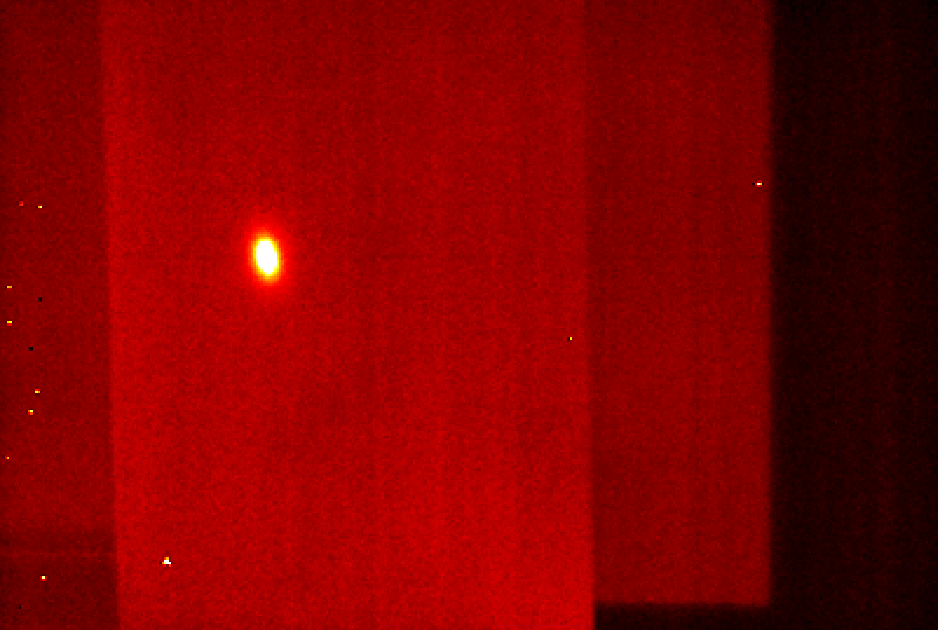
\includegraphics[width=0.3\linewidth]{fig10cc.png}} \hfill
  \subfigure[]{\label{subfig:10d}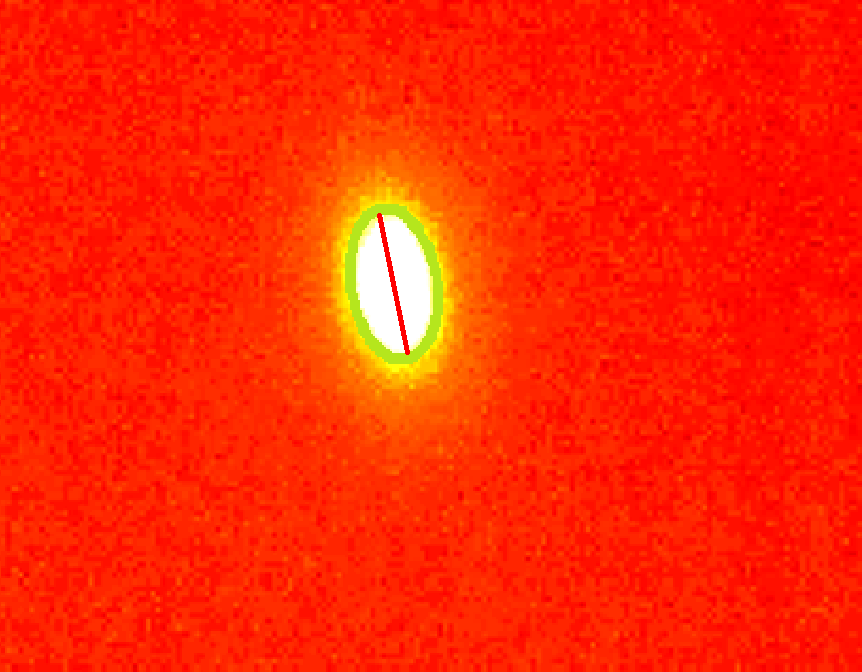
\includegraphics[width=0.3\linewidth]{fig10dd.png}}
  \hspace*{\fill}
	
	\caption{Example of fiber orientation detection: (a)-(b) horizontally oriented - (c)-(d)
		vertically oriented.}
		\label{fig:10}
		\end{figure}
